\section{Análisis de resultados}\label{sec:resultados}

La evaluación se hizo con tres fuentes complementarias, todas reproducibles con \texttt{python pruebas/evaluacion.py} (semilla fija):

\begin{enumerate}
    \item \textbf{Casos de prueba} con el horario real del estudiante, con entradas y salidas esperadas y obtenidas (sección~\ref{sec:mejores}).
    \item \textbf{Simulación de \resEscenarios\ escenarios aleatorios} (de 4 a 7 materias, laboratorios, entregas y disponibilidades distintas), donde se verifican las restricciones del plan y se compara con una estrategia de referencia (sección~\ref{sec:significativo}).
    \item \textbf{Usuarios simulados} para medir si la calibración mejora las estimaciones (sección~\ref{sec:calibracion}).
\end{enumerate}

Además, el sistema cuenta con \resPruebas\ pruebas automáticas (del motor, la validación, las recomendaciones, la calibración, el progreso, el asistente y la API) que pasan todas. Las del asistente comprueban que las respuestas sobre el horario salen de los datos del estudiante, que cada método citado tiene referencias, que la entrevista produce un plan personal y que el sistema funciona completo sin el modelo de lenguaje.

\textbf{Alcance de la evaluación del asistente.} Las pruebas del asistente son funcionales y verifican su parte determinista. No se midió la calidad de las respuestas del modelo de lenguaje opcional (solo se revisaron casos a mano, con errores corregidos mediante la instrucción restringida) ni si los métodos recomendados mejoran el rendimiento de las personas; eso requiere una evaluación con usuarios.

\subsection{Los dos mejores casos de prueba}\label{sec:mejores}

\subsubsection{Caso CP1: semana base del estudiante}

Es el caso de referencia: el horario real del estudiante y tres trabajos registrados (Parcial 2 de ECDI, entrega 1 de ARSW y Hito 2 de PTIA), consultado el lunes 12 de octubre de 2026 a las 9:00. El sistema generó \resBloquesBase\ bloques: \resHTareasBase\ horas en tareas y \resHEstudioBase\ horas de estudio independiente en el horizonte. La tabla~\ref{tab:cp1} compara lo esperado con lo obtenido y la figura~\ref{fig:carga} muestra la carga por día.

\textbf{Entrada.} Horario real del equipo (6 materias, 14 bloques), 3 trabajos registrados, lunes 12/10/2026 09:00 (semana 8, par).

\begin{table}[H]
\centering\small
\caption{Caso CP1: Semana base del equipo}\label{tab:cp1}
\begin{tabularx}{\textwidth}{>{\raggedright\arraybackslash}X >{\raggedright\arraybackslash}p{3.3cm} >{\raggedright\arraybackslash}p{3.3cm} c}
\toprule
Comprobación & Esperado & Obtenido & ¿Cumple? \\
\midrule
Tareas con tiempo asegurado & 15 de 15 & 15 de 15 & Sí \\
Violaciones de restricciones duras & 0 & 0 & Sí \\
Máximo de horas en un día & $\leq$ 6 h & 6 h & Sí \\
Parcial difícil (entrega 20/10) termina con $\geq$ 2 días de colchón & último bloque $\leq$ 18/10 & último bloque 16/10 & Sí \\
Advertencias de tiempo & 0 & 0 & Sí \\
\bottomrule
\end{tabularx}
\end{table}


\begin{figure}[H]
\centering
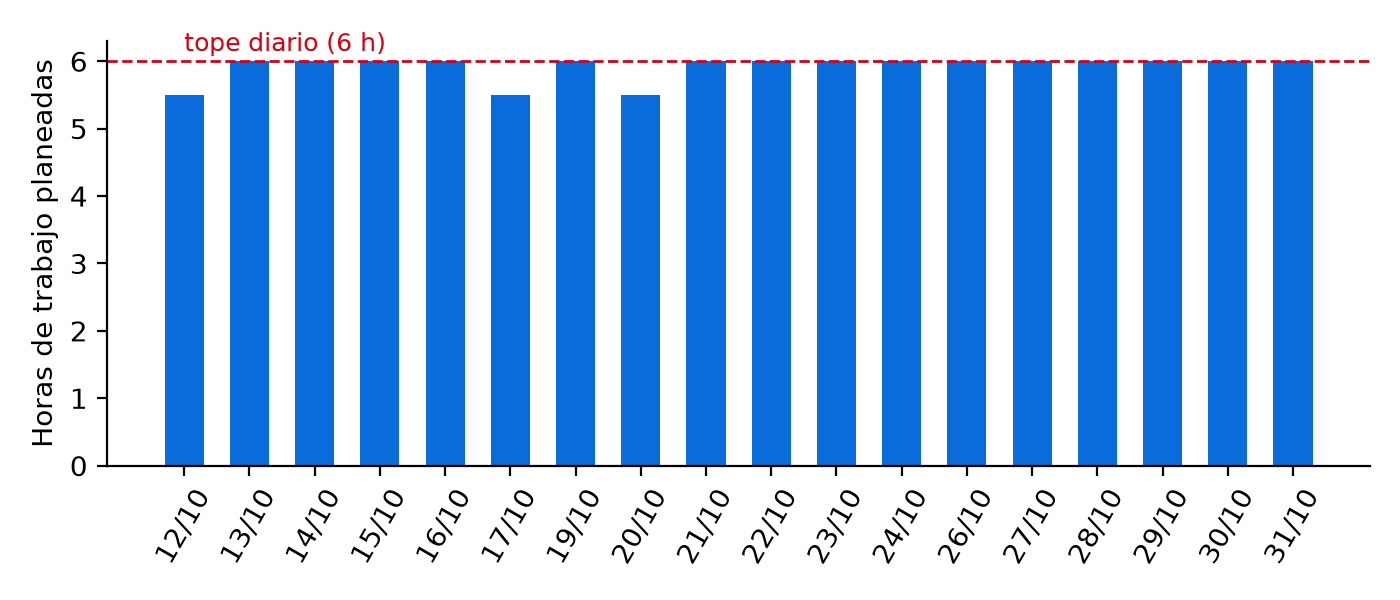
\includegraphics[width=0.8\textwidth]{img/fig_carga_dia.png}
\caption{Horas de trabajo por día en el caso CP1; ningún día supera el tope de 6 horas}\label{fig:carga}
\end{figure}

El resultado cumple todo lo esperado. El máximo de 6 horas coincide con el tope configurado, lo que muestra que el límite actúa (varios días lo alcanzan) sin ser superado. El parcial difícil, con entrega el 20 de octubre, termina el 16, es decir, con más de los dos días de margen que le corresponden por su dificultad.

\subsubsection{Caso CP3: marcar tareas como hechas}

Muestra el recálculo del plan, una función central del MVP. Partiendo del caso base, el estudiante marca como hechos el parcial y el informe de laboratorio de ARSW.

\textbf{Entrada.} Caso base; el estudiante marca como hechos el Parcial 2 de ECDI y el informe de laboratorio de ARSW (09/10).

\begin{table}[H]
\centering\small
\caption{Caso CP3: Marcar tareas como hechas reacomoda el plan}\label{tab:cp3}
\begin{tabularx}{\textwidth}{>{\raggedright\arraybackslash}X >{\raggedright\arraybackslash}p{3.3cm} >{\raggedright\arraybackslash}p{3.3cm} c}
\toprule
Comprobación & Esperado & Obtenido & ¿Cumple? \\
\midrule
Desaparecen los bloques de las tareas hechas & 0 bloques & 0 bloques & Sí \\
Baja el trabajo en tareas & $<$ 53,5 h & 41,5 h & Sí \\
El tiempo liberado pasa a estudio independiente & > 53 h & 64,5 h & Sí \\
Las demás tareas siguen cubiertas & 13 de 13 & 13 de 13 & Sí \\
\bottomrule
\end{tabularx}
\end{table}


Las dos tareas desaparecen del plan y el tiempo que ocupaban se reasigna a estudio independiente, que es lo que se espera: avanzar en las metas de estudio de cada materia en lugar de dejar huecos sin uso. Ninguna otra tarea pierde su tiempo.

\subsubsection{Otros casos}

Cuatro casos más completan la evaluación. El caso CP2 (entrega imposible) comprueba el comportamiento ante una tarea que no cabe: el sistema la advierte, dice que faltan \resFaltanImposible\ horas, respeta el tope diario y no afecta a los demás trabajos. El caso CP4 comprueba que un día sin disponibilidad se respeta, y el caso CP5 que la calibración aumenta las estimaciones sin tocar las horas que el estudiante fijó (con 5 talleres registrados que tomaron 1,5 veces lo estimado, el factor aprendido es \resFactorTaller, cercano a 1,5 pero sin igualarlo, como se diseñó). El caso CP6 comprueba el asistente sin modelo de lenguaje: responde la agenda de hoy con la clase y el bloque reales, pone primero el parcial cuando se pregunta por él, termina el plan de repasos en la fecha de la entrega, no inventa ante una pregunta fuera de tema, arma el plan personal tras la entrevista (con el sueño primero cuando se duerme menos de 6 horas) y puede explicar las \resNRecomendaciones\ recomendaciones del plan.

\textbf{Entrada.} Caso base + un proyecto difícil de 40 h que se entrega mañana (13/10).

\begin{table}[H]
\centering\small
\caption{Caso CP2: Entrega imposible}\label{tab:cp2}
\begin{tabularx}{\textwidth}{>{\raggedright\arraybackslash}X >{\raggedright\arraybackslash}p{3.3cm} >{\raggedright\arraybackslash}p{3.3cm} c}
\toprule
Comprobación & Esperado & Obtenido & ¿Cumple? \\
\midrule
Advertencia «no alcanza el tiempo» para el proyecto & 1 advertencia & 1 advertencia(s) & Sí \\
Horas asignadas + horas que faltan = 40 h & 40 h & 8 + 32 = 40 h & Sí \\
Se respeta el tope diario pese a la presión & 0 violaciones & 0 violaciones & Sí \\
Los demás trabajos registrados siguen cubiertos & 3 de 3 & 3 de 3 & Sí \\
\bottomrule
\end{tabularx}
\end{table}

\textbf{Entrada.} Caso base pero el sábado deja de estar disponible.

\begin{table}[H]
\centering\small
\caption{Caso CP4: Se respeta un día sin disponibilidad}\label{tab:cp4}
\begin{tabularx}{\textwidth}{>{\raggedright\arraybackslash}X >{\raggedright\arraybackslash}p{3.3cm} >{\raggedright\arraybackslash}p{3.3cm} c}
\toprule
Comprobación & Esperado & Obtenido & ¿Cumple? \\
\midrule
Bloques el sábado & 0 & 0 & Sí \\
Violaciones de restricciones duras & 0 & 0 & Sí \\
Tareas cubiertas o advertidas (sin fallas silenciosas) & 100 \% & 15 cubiertas, 0 advertidas de 15 & Sí \\
\bottomrule
\end{tabularx}
\end{table}

\textbf{Entrada.} Caso base; el estudiante registró 5 talleres que estimados en 2 h le tomaron 3 h (razón 1,5).

\begin{table}[H]
\centering\small
\caption{Caso CP5: La calibración ajusta las estimaciones}\label{tab:cp5}
\begin{tabularx}{\textwidth}{>{\raggedright\arraybackslash}X >{\raggedright\arraybackslash}p{3.3cm} >{\raggedright\arraybackslash}p{3.3cm} c}
\toprule
Comprobación & Esperado & Obtenido & ¿Cumple? \\
\midrule
Sin historial el factor es 1 (el plan no cambia) & 1,00 & 1,00 & Sí \\
Con 5 registros el factor se acerca a 1,5 sin igualarlo & entre 1,30 y 1,50 & 1,42 & Sí \\
Aumentan los minutos asignados a talleres & > 630 min & 990 min & Sí \\
Los trabajos con horas fijadas por el estudiante no cambian & 480 min (PTIA) & 480 min & Sí \\
\bottomrule
\end{tabularx}
\end{table}

\textbf{Entrada.} Caso base, sin modelo de lenguaje: preguntas «¿Qué tengo hoy?», «¿cuándo es mi parcial?», «¿cómo estudio para el parcial de ECDI?», una pregunta fuera de tema y la entrevista de cinco preguntas.

\begin{table}[H]
\centering\small
\caption{Caso CP6: El asistente responde con los datos del estudiante}\label{tab:cp6}
\begin{tabularx}{\textwidth}{>{\raggedright\arraybackslash}X >{\raggedright\arraybackslash}p{3.3cm} >{\raggedright\arraybackslash}p{3.3cm} c}
\toprule
Comprobación & Esperado & Obtenido & ¿Cumple? \\
\midrule
«¿Qué tengo hoy?» muestra la clase y el bloque reales del lunes 12/10 & 09:00–11:00 y Taller MATE ECDI & ambos presentes & Sí \\
«¿Cuándo es mi parcial?» pone primero el parcial con su fecha & Parcial 2 de ECDI, 20/10 & Parcial 2 de ECDI, 20/10 & Sí \\
El plan de repasos termina en la fecha de la entrega & martes 20/10 & martes 20/10 & Sí \\
Una pregunta fuera de tema no se inventa & «No tengo una respuesta segura» & sin respuesta inventada & Sí \\
La entrevista arma el plan personal y pone primero el sueño (duerme menos de 6 h) & Dormir como parte del estudio & primero & Sí \\
Cada recomendación se puede explicar en el chat & 11 de 11 & 11 de 11 & Sí \\
\bottomrule
\end{tabularx}
\end{table}


\subsection{El caso más significativo: comparación con la estrategia de último momento}\label{sec:significativo}

El caso más revelador no es una situación puntual sino la comparación del plan con lo que haría un estudiante sin planeación. Se simuló una estrategia de referencia de \emph{último momento}: cada trabajo se hace lo más tarde posible, hacia atrás desde su entrega, sin tope diario ni margen, usando los mismos huecos libres. Ambas estrategias se aplicaron a los mismos \resEscenarios\ escenarios aleatorios (\resTareas\ trabajos en total). Sobre el plan de SemestrIA se verificaron además nueve tipos de restricción dura.

\textbf{Entradas.} Escenarios generados con semilla fija: de 4 a 7 materias, horarios con laboratorios semanales o quincenales, de 2 a 7 trabajos con entregas de 2 a 28 días y disponibilidad variable (incluidos sábados y domingos).

\textbf{Salidas esperadas.} Cero violaciones de restricciones y cero fallas silenciosas; menos días sobrecargados y menos trabajos terminados el día de la entrega que la estrategia de último momento.

\textbf{Salidas obtenidas.} Se obtuvieron \resViol\ violaciones en los \resEscenarios\ escenarios y la tabla~\ref{tab:comparacion} y la figura~\ref{fig:comparacion} comparan las estrategias.

\begin{table}[H]
\centering\small
\caption{Comparación contra la estrategia de último momento (300 escenarios)}\label{tab:comparacion}
\begin{tabular}{lrr}
\toprule
Métrica & Último momento & SemestrIA \\
\midrule
Trabajos con tiempo asegurado (\%) & 99,7 & 98,4 \\
Días con más de 6 h de trabajo, por escenario & 1,71 & 0,0 \\
Máximo de horas en un día (promedio) & 8,35 & 5,84 \\
Trabajos terminados el mismo día de la entrega (\%) & 90,1 & 5,1 \\
Anticipación media respecto a la entrega (días) & 0,15 & 7,53 \\
\bottomrule
\end{tabular}
\end{table}


\begin{figure}[H]
\centering
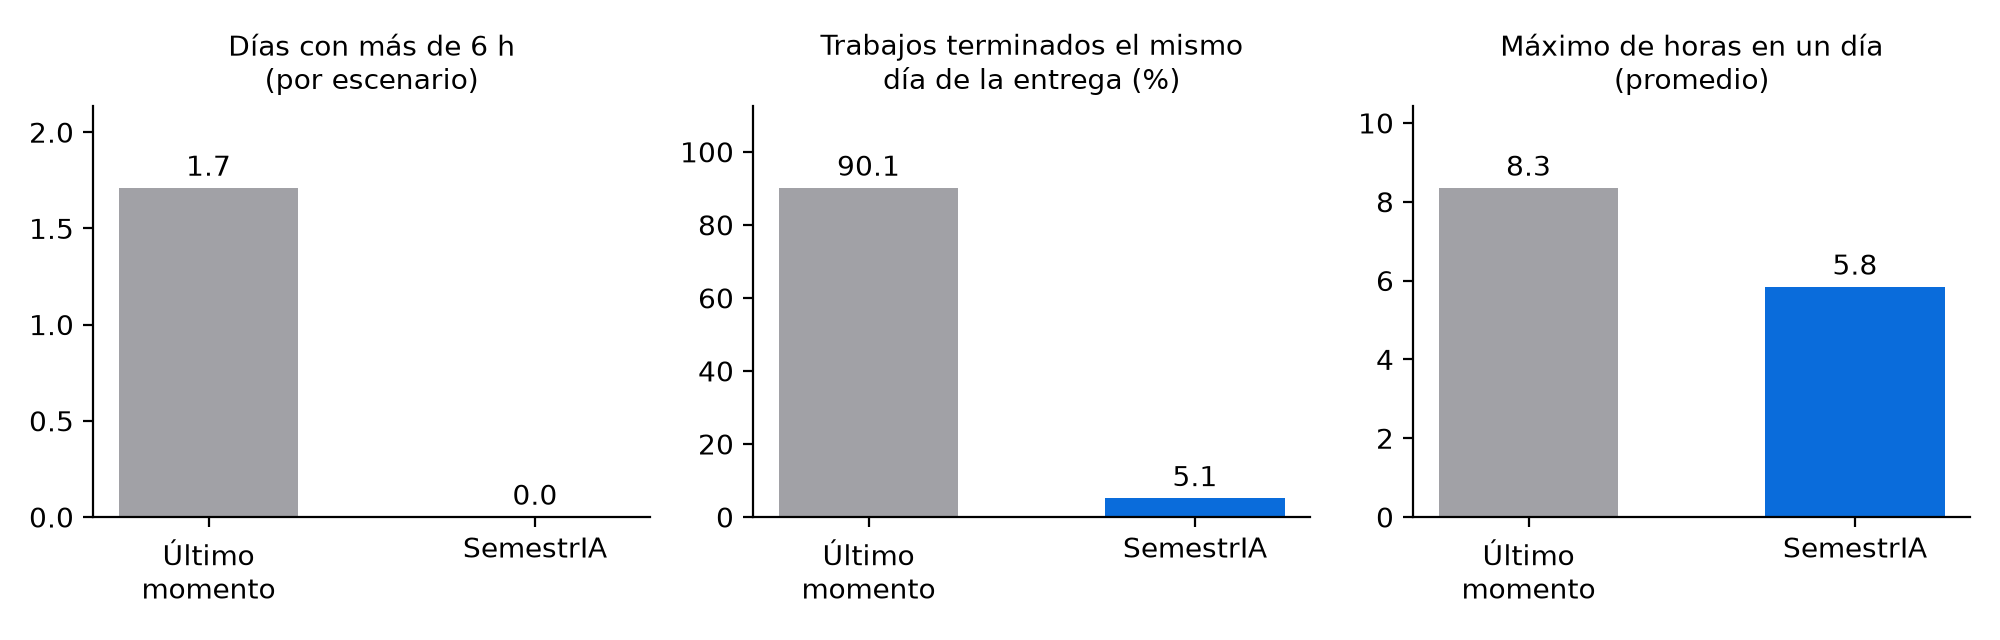
\includegraphics[width=\textwidth]{img/fig_comparacion.png}
\caption{SemestrIA frente a la estrategia de último momento en los escenarios simulados}\label{fig:comparacion}
\end{figure}

\textbf{Análisis.}
\begin{itemize}
    \item \textbf{La carga se reparte.} La estrategia de último momento produce en promedio \resDiasSobreUlt\ días por escenario con más de 6 horas de trabajo y un día pico de \resMaxUlt\ horas; el plan de SemestrIA no tiene ningún día sobrecargado y su día pico promedia \resMaxEdf\ horas. Esto refleja el efecto del tope diario y del límite por tarea.
    \item \textbf{Hay margen.} Con la estrategia de último momento el \resColUlt\,\% de los trabajos se termina el mismo día de la entrega, frente al \resColEdf\,\% con SemestrIA (una reducción del \resRedCol\,\%); los trabajos se terminan en promedio \resAntEdf\ días antes de su fecha, frente a \resAntUlt\ días.
    \item \textbf{Hay un costo.} La estrategia de último momento deja con tiempo completo al \resPctCubUlt\,\% de los trabajos y SemestrIA al \resPctCub\,\%. La diferencia es la consecuencia directa de los topes de bienestar: sin límite se logra algo más de cobertura a costa de jornadas de más de 8 horas. En \resConAdv\ de los \resEscenarios\ escenarios algún trabajo no cabe, y en todos esos casos el sistema lo advirtió (cero fallas silenciosas): el estudiante se entera con tiempo de que debe negociar un plazo o ajustar su disponibilidad.
    \item \textbf{Rapidez.} Cada plan tarda en promedio \resMsMedia\ ms (percentil 95: \resMsPNov\ ms; máximo: \resMsMax\ ms), por lo que se recalcula al instante con cada cambio.
\end{itemize}

\textbf{Límites de la comparación.} La estrategia de último momento es un modelo del comportamiento de un estudiante, no una medición de personas reales, y los escenarios son sintéticos. Los resultados muestran que el plan cumple lo que se diseñó que cumpliera, pero no demuestran que los estudiantes rindan más con él; eso exige una evaluación con usuarios, que no se hizo (sección~\ref{sec:conclusiones}).

\subsection{Calibración de las estimaciones}\label{sec:calibracion}

Para medir si aprender de las horas reales mejora las estimaciones, se simularon \resUsuarios\ estudiantes por cada ritmo (0,6; 0,8; 1; 1,3; 1,6 y 2 veces la estimación base, con ruido aleatorio), cada uno con 12 trabajos. Se comparó el error absoluto medio entre la estimación y las horas reales en los trabajos 6 a 12, con la estimación base y con la calibrada con los registros anteriores.

\begin{table}[H]
\centering\small
\caption{Error de estimación con y sin calibración (usuarios simulados)}\label{tab:calibracion}
\begin{tabular}{rrrr}
\toprule
Ritmo real vs. base & Error base (h) & Error calibrado (h) & Reducción \\
\midrule
0.6$\times$ & 1,69 & 0,52 & 69,0\,\% \\
0.8$\times$ & 0,94 & 0,64 & 32,1\,\% \\
1$\times$ & 0,7 & 0,73 & -4,3\,\% \\
1.3$\times$ & 1,48 & 0,97 & 34,9\,\% \\
1.6$\times$ & 2,78 & 1,31 & 52,8\,\% \\
2$\times$ & 4,57 & 1,74 & 61,9\,\% \\
\bottomrule
\end{tabular}
\end{table}


\begin{figure}[H]
\centering
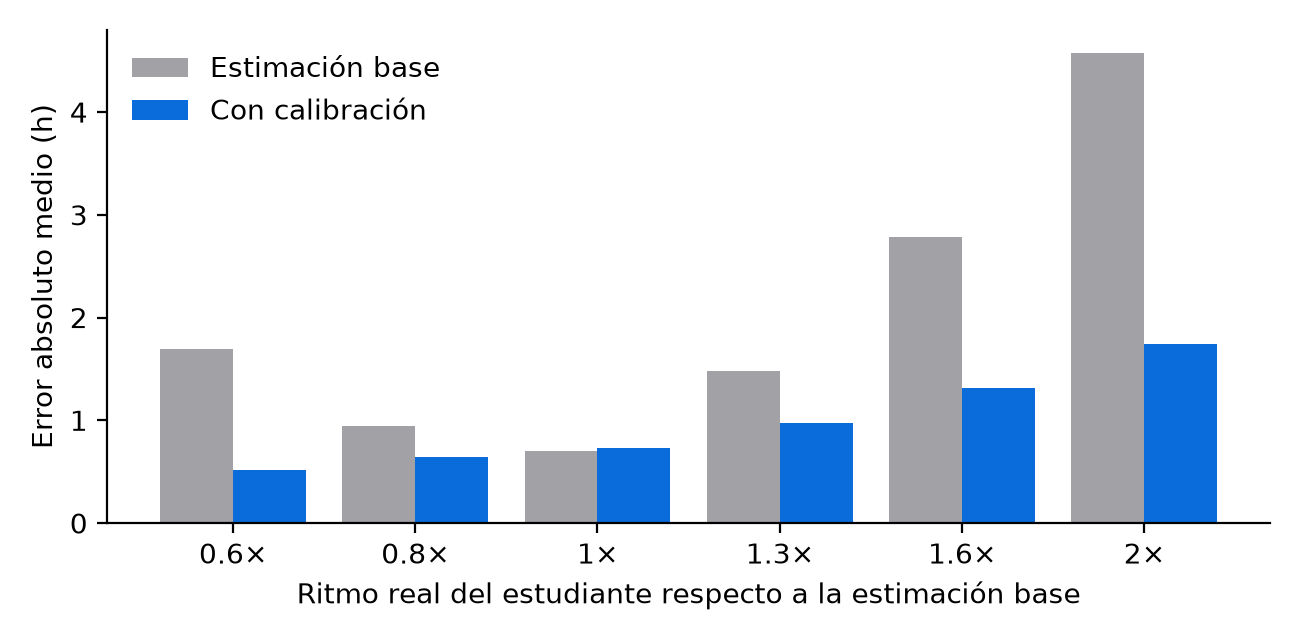
\includegraphics[width=0.75\textwidth]{img/fig_calibracion.png}
\caption{Error de estimación con y sin calibración según el ritmo real del estudiante}\label{fig:calibracion}
\end{figure}

La calibración reduce el error en promedio un \resRedCalSes\,\% para los estudiantes cuyo ritmo difiere de la estimación base, y más cuanto mayor es la diferencia (hasta cerca de 70\,\% para quien trabaja más rápido de lo estimado). Hay un costo pequeño: para quien ya coincide con la estimación base (ritmo de 1) el error empeora un \resCalUnoAbs\,\%, porque el factor aprendido oscila alrededor de 1 por el ruido de las observaciones. La reducción media sobre todos los ritmos es del \resRedCalMedia\,\%. Estos resultados provienen de usuarios simulados y dependen del ruido supuesto.

\subsection{Cumplimiento de los criterios de aceptación}

La tabla~\ref{tab:objetivos} contrasta los criterios definidos en la sección~\ref{sec:alcance} con los resultados.

\begin{table}[H]
\centering\small
\caption{Cumplimiento de los criterios de aceptación del MVP}\label{tab:objetivos}
\begin{tabularx}{\textwidth}{l >{\raggedright\arraybackslash}X r r c}
\toprule
 & Criterio & Umbral & Resultado & ¿Cumple? \\
\midrule
OC1 & Restricciones duras violadas en los escenarios simulados & 0 & 0 & Sí \\
OC2 & Fallas silenciosas (trabajo sin tiempo completo y sin advertencia) & 0 & 0 & Sí \\
OC3 & Tiempo de planificación, percentil 95 & $\leq$ 100 ms & 4,76 ms & Sí \\
OC4 & Días con más de 6 h de trabajo (vs. último momento) & 0 & 0 & Sí \\
OC5 & Reducción de trabajos terminados el día de la entrega & $\geq$ 50 \% & 94,3 \% & Sí \\
OC6 & Trabajos con tiempo asegurado en escenarios aleatorios & $\geq$ 95 \% & 98,4 \% & Sí \\
OC7 & Reducción del error de estimación (ritmo real distinto de la base en al menos 20 \%) & $\geq$ 25 \% & 32,1 \% a 69,0 \% & Sí \\
OC8 & Pruebas automáticas que pasan & 100 \% & 73 de 73 & Sí \\
\bottomrule
\end{tabularx}
\end{table}

